\section{Modellbildung des UR10}

Für die erste Aufgabe soll der Roboter in der Matlab Simulationssoftware Simscape modelliert werden.
Anders als in der Aufgabenstellung angegeben, gibt es für den UR10 lediglich eine step-Datei über den gesamten Roboter und nicht aufgeteilt in die einzelnen Armteile als Download.


\subsection{Download und Konvertierung der step-Dateien}
Die step-Datei des UR10 wird auf diversen Webseiten kostenlos zum Download angeboten.
Für das Projekt wurde die Datei der Firma \en{SG-Automatisierungstechnik GmbH}\footnote{\url{https://www.sg-automation.at/}} verwendet.
Die step-Datei lässt sich jedoch nicht direkt in Matlab einlesen, sondern muss mittels des \en{Simscape Multibody Link Plugin} konvertiert werden.
Dabei handelt es sich um ein Zusatzprogramm, welches in bestimmten CAD Anwendungen installiert werden kann und den Export von XML- und Geometriedateien ermöglicht \cite{sm_plugin}.
Als CAD Anwendung für die Konvertierung wurde SolidWorks gewählt. 
Der Dateiexport aus SolidWorks erzeugte eine XML-Datei, eine Geometriedatei \en{UR10\_DataFile.m} sowie acht step-Dateien der einzelnen Armteile und der Basis.


\subsection{Modellierung in Simscape}

Nun kann die XML-Datei mittels dem Befehl \en{sm\_import()} in Matlab Simscape eingelesen und mit den step-Dateien der Roboterbauteile verknüpft werden.
Nach einer kurzen Sichtung des Modells stellte sich heraus, dass die Transformationen zwischen den Bauteilen zwar korrekt, jedoch die interne Verknüpfung nicht stimmig war.
Beim Einfügen von Aktuatoren bewegte sich ausschließlich das angesteuerte Armteil, während der Rest der kinematischen Kette statisch in der Ausgangsposition verblieb. 

Aus diesem Grund wurde der Import einer URDF-Datei des Roboters versucht, was ebenso über den Befehl \en{sm\_import()} möglich ist.
Die verwendete Datei kann aus dem Github-Repository von \en{Positronics Lab}\footnote{\url{https://github.com/PositronicsLab}}, einer Forschungsorganisation der George Washington Universität, kostenlos heruntergeladen werden.
Hierbei erzeugt Matlab eine eigene XML-Datei, in welcher das Projekt gespeichert ist.
Mit Einfügen der step-Dateien der Armteile erhält man ein funktionierendes Robotermodell des UR10.
Die Massen und Trägheiten der Armteile wurden aus der zuvor erhaltenen Geometriedatei entnommen.



\subsection{Festlegung der Roboterkoordinatensysteme nach Denavit-Hartenberg-Konvention}

Für die spätere Vergleichsrechnung mit dem Newton-Euler-Verfahren ist es von Vorteil die Koordinatensysteme der Gelenkachsen des Roboters einheitlich zu definieren. %eine einheitliche Festlegung der Koordinatensysteme des Roboters zu definieren.
Hierzu bietet sich die Festlegung nach Denavit-Hartenberg-Konvention an.
Die nachfolgende Abbildung \ref{fig:ur10_dh} zeigt die Koordinatensysteme, wie sie auch in der Simulation definiert sind.

\begin{figure}[!htbp]
	\centering
	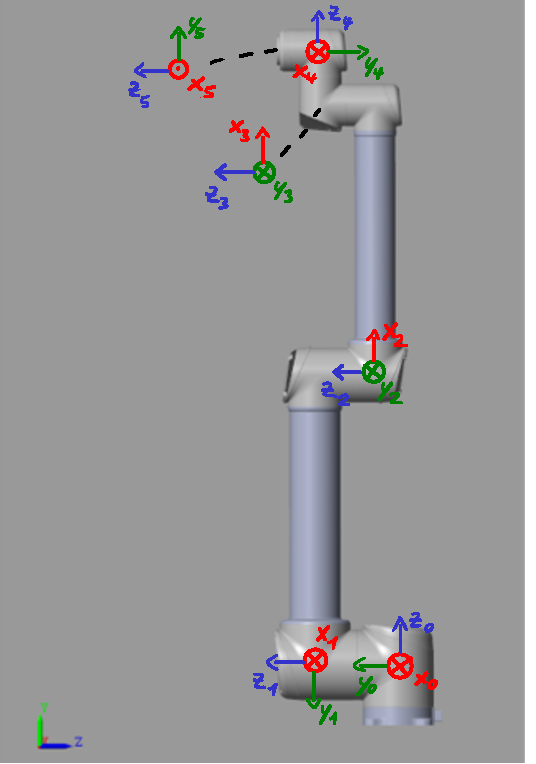
\includegraphics[width=0.5\linewidth]{grafic/Bild1.pdf}
	\caption{Koordinatensysteme der Gelenke des Roboters nach Denavit-Hartenberg-Konvention}
	\label{fig:ur10_dh}
\end{figure}


